% !TeX encoding = UTF-8

\chapter{REVISÃO BIBLIOGRÁFICA}\label{ch:rev-bibs}

Vários trabalhos serviram como fonte de conhecimento e suporte para o entendimento e desenvolvimento deste tema. Alguns foram considerados mais importantes por abordar detalhadamente o problema de reconhecimento, outros foram buscados para se entender melhor, ou ter outra visão sobre algum detalhes específico do problema.

Trabalhos de autores como \cite{geysilva} ajudaram a estruturar e organizar o tema por abordar tópicos similares e por possuir riqueza de detalhes no assunto de análise de componentes apresentando uma implementação em \textit{MatLab} (um \textit{software} interativo voltado para o cálculo numérico).

O trabalho de \cite{img-digital-willians} foi utilizado para se aprofundar no tema de imagens digitais, assim como  \cite{gonzalez_woods} que também esclareceu o funcionamento de escalonamento, normalização e mono cromatização de imagens. O autor Dr. Andrew Davison em seus trabalhos, dentre os quais, \cite{drmathew_java_programming} se destacou pela ótima didática facilitando o entendimento de Análise de Componentes e sua relação com \textit{EigenFaces}, disponibilizando ainda exemplos de implementação em \textit{JAVA}. 

Os trabalhos \cite{tutorial_en_smith} e \cite{tutorial_pt} foram estudados como tutoriais do processo de ACP e será usado posteriormente como guias de implementação do algorítimo.

Nas próximas seções serão explanados os conteúdos destes e de outros trabalhos disponibilizados em uma ordem didática.


\section{AQUISIÇÃO E PROCESSAMENTO DE IMAGENS E VÍDEO}\label{sec:processamento_imagens}

Com a abrangência dos sistemas de comunicação, com difusão de conhecimentos informações pelos diversos meios, captar, armazenar e processar imagens se tornou necessidade fundamental. Para o reconhecimento de faces em vídeo, o sucesso deste processo é pré-requisito  para o funcionamento dos algoritmos. 

As sessões a seguir contemplam fundamentos básicos sobre imagem, vídeo, a alguns de seus processamentos necessários para a aplicação dos algoritmos de detecção e reconhecimento de faces.


\subsection{IMAGEM E VÍDEO DIGITAL}\label{subsec:imagem}

A imagem digital são valores numéricos disponibilizados em uma matriz bidimensional. Basicamente existem dois tipos de imagens: os chamados \textit{rasters} ou \textit{bitmaps}, e vetorizadas. A primeira são representações de cada ponto da imagem com alguma cor usadas geralmente em fotografias, enquanto que o segundo é produzido por plotadores que recebem os pontos e as distâncias entre eles como parâmetros, consideranto retas, curvas, polígonoas e etc, sendo assim não perdem sua qualidade quando redimensionados.

Converter uma imagem para o formato digital significa transferir os elementos que a compõem para elementos representativos de cada pequeno fragmento original. O menor elemento da imagem, o \textit{pixel}, é identificado segundo sua intensidade de nível de cinza e as cores correspondentes. Identificados, estes elementos são armazenados por códigos que podem ser reconhecidos pelo dispositivo de visualização e apresentados novamente por um dispositivo de visualização, como um monitor de vídeo ou impressora \cite{img-digital-willians}. 

%\vspace*{13cm}
\begin{figure}[h]
	\centering
	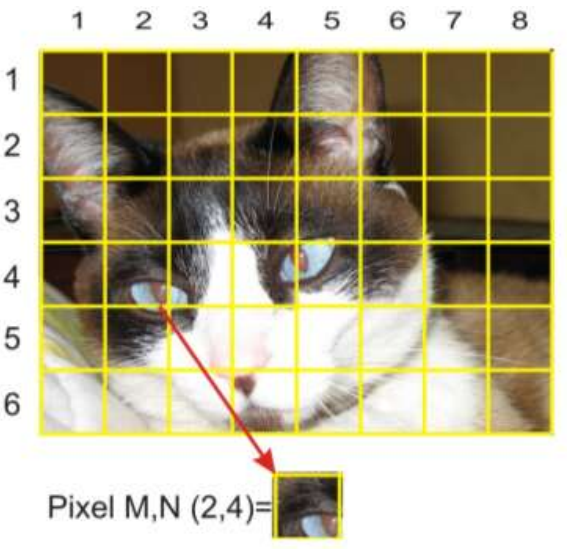
\includegraphics[width=.6\textwidth]{pixel-img}
	\caption{Exemplo de imagem representada como uma matriz (M,N) de pixels, com destaque para o pixel (2,4).}
	\fonte{\cite{img-digital-willians}}
	\label{pixel_img}
\end{figure}



Uma imagem analógica que é a (representação real da cena, para ser convertida para o formato do
processamento computacional deve sofrer uma separação espacial (amostragem) e em amplitude
(quantização) \cite{img-digital-willians}. 

A amostragem é a divisão do plano x,y em uma grade (ou matriz bi dimensional) onde x e y serão números inteiros. Os pontos da matriz de são denominados \textit{pixels} (\textit{PICTure Elements}), como ilustra a \autoref{pixel_img}. Cada pixel representa uma parte da cena real, desta forma a resolução espacial da imagem é proporcional aos valores de M e N correspondentes na matriz (exemplo Fig.22). Em geral a malha de amostragem, o formato dos pixels (x,y), é retangular, mas pode também ser triangular ou mais complexa. Os valores de cada ponto da matriz, coluna x linha (xy), que identifica um único pixel (M,N0, devem ser escolhidos de forma a respeitar a relação qualidade da imagem x espaço de armazenamento, em função da aplicação para a qual a imagem se destina. Para uma imagem digital com 256 níveis de cinza o número de bytes ocupados para armazenar a imagem é o produto da linha vezes a coluna da matriz \cite{img-digital-willians}. 

Matematicamente, toda imagem monocromática (preto e branco) é um função f(x,y) da intensidade luminosa, em qualquer parte das coordenadas (x,y), proporcional ao brilho (tons de cinza) da imagem em um determinado ponto. A figura mostra uma imagem e como representamos os eixos x e y no plano cartesiano \cite{gonzalez_woods}. 

A função  f(x,y)  é a multiplicação da iluminância  i(x,y) (que é a quantidade de luz que incide sobre o objeto) pela refletância  r(x,y)  (que é fração de luz incidente que o objeto vai refletir ao ponto (x,y). 

Sendo assim, podemos dizer que :

f(x,y) = i(x,y) * r(x,y),

onde 0 < i(x,y) e 0 < r(x,y) < 1 .

Quando se utiliza uma imagem colorida, no padrão RGB por exemplo,  deve se usar uma função f(x,y) para cada banda, R(Red), G(Green) e B(Blue) que são as cores primárias\cite{gonzalez_woods}.


\subsection{FORMATO PNG}\label{subsec:png}

O PNG (\textit{Portable Network Graphics} ou "\textit{PNG is Not Giff}") é um formato de representação de imagens do tipo \textit{rasters}. foi desenhado para substituir o formato GIF e o TIFF em certa extensão. O PNG tem 3 vantagens principais: suporta canal alfa (transparência) de forma eficiente, tem a maior gama de profundidade de cores e alta compressão que pode ser regulável. Além disso, o formato é livre enquanto os outros possuem patentes \cite{png}. 

O trabalho da compressão é justamente retirar essas informações redundantes para diminuir o peso do arquivo. Por exemplo, vamos imaginar um pixel qualquer de uma imagem. Possivelmente, a cor ou o valor desse pixel será igual a de vários outros elementos dentro da mesma imagem. Quando a imagem é comprimida, em vez de ela possuir vários pixels iguais e repetidos, ela guarda apenas um valor desse pixel, que é reproduzido para os outros semelhantes, economizando tempo de carregamento \cite{img_compact}. Outras técnicas mais complexas também são utilizadas.

Este formato leve e de fácil manipulação foi escolhido neste trabalho para a representação de imagens digitais quando for necessário.


\subsection{AQUISIÇÃO DE IMAGEM E VÍDEO}\label{subsec:aquisicao_video}

No processo de aquisição de imagens, tradicionalmente, um uma "cena" tridimensional (ou imagem analógica) deve ser capturada por um dispositivo eletrônico, que colhe uma amostragem convertendo-a para uma imagem digital de duas dimensões. Por exemplo, uma câmera digital captando uma cena 3D e convertêndo-a em 2D.

Atualmente o dispositivo de conversão mais usado  é a câmera CCD (\textit{charge coupled device}), que é uma matriz de células semi-condutoras fotossensíveis que trabalham com capacitadores, fazendo um armazenamento da carga elétrica proporcional à energia luminosa incidente \cite{gonzalez_woods}.

A saída deste processo é a imagem do tipo \textit{raster}, pronta pra ser formatada e compactada por alguma representação (PNG, JPG, BPM, etc). 

\subsection{PROCESSAMENTO DE IMAGEM}\label{subsec:processamento}

O processamento de imagem é todo o processo que tem uma imagem como entrada e saída, tais como fotografia ou quadros de vídeo. 

Usa-se para melhorar o aspecto visual de certas feições estruturais para o analista humano ou para performance e para fornecer outros subsídios para a sua interpretação, inclusive gerando produtos que possam ser posteriormente submetidos a outros processamentos \cite{inpe_proc_img}.

O processamento de imagens pode ser dividido em 3 fases básicas: pré-processamento, realce e classificação.
Pré-processamento refere-se ao processamento inicial de dados brutos para calibração radiométrica da imagem, correção de distorções geométricas e remoção de ruído.
Realce visa melhorar a qualidade da imagem, permitindo uma melhor discriminação dos objetos presentes na imagem.
Na classificação são atribuídas classes aos objetos presentes na imagem \cite{inpe_proc_img}.

Nas próximas seções algumas técnicas de processamento de imagens serão abordadas pela sua importância e sua necessidade de uso em algorítimos de detecção e reconhecimento de faces. São elas:

\begin{itemize}
	\item Conversão em Escala de Cinza: considerada uma técnica pré-processamento, é usada para transformar a imagem em "preto e branco" (na escala de cinza) , o que torna outras operações de processamento mais rápidas e eficientes;
	\item Escalonamento: pré-processamento de correção linear geométrica 2D \cite{lapix_escala};
	\item Equalização: uma técnica de realce de contraste \cite{gonzalez_woods}
	\item Segmentação: recorte da imagem, onde se extraem os objetos relevantes para a aplicação desejada \cite{inpe_proc_img}.
	\item Classificação: uso de classificadores para reconhecer padrões em imagens \cite{drmathew_java_programming}
\end{itemize}

\subsubsection{CONVERSÃO EM ESCALA DE CINZA}\label{subsubsec:filtros}

Em fotografia, computação e colometria, uma imagem em escala de cinza é uma imagem em que cada valor de pixel é uma única amostra da representação de intensidade de luz \cite{stephen_greyscale}. Em outras palavras, o valor R, G e B de cada pixel devem ser iguais para se obter uma escala de cinza que varia de preto em sua intensidade mais baixa para o branco absoluto.

A conversão de uma cor para escala de cinza não é algo único. Existem diversas maneiras e possivilidades de inserção de parametros que dariam resultados diferentes. A maneira mais usual é calcular a média dos valores RGB de cadca pixel e atribuir o resultado ao pixel novamente. Exemplo:

Gray = (Red + Green + Blue) / 3, reconhecendo que o algorítimo na verdade seria algo como:

For Each Pixel in Image {
	
	Red = Pixel.Red
	Green = Pixel.Green
	Blue = Pixel.Blue
	
	Gray = (Red + Green + Blue) / 3
	
	Pixel.Red = Gray
	Pixel.Green = Gray
	Pixel.Blue = Gray
	
}

Converter a imagem em escala de é necessário para tornar eficientes os subsequente processos, como equalização e aplicação de classificadores \cite{drmathew_java_programming}.


\subsubsection{ESCALONAMENTO}\label{subsubsec:escalonamento}

O escalonamento de imagens é uma transformação geométrica 2D. Pontos no Plano xy podem ser escalonados (esticados) por fatores de escala Sx e Sy através de multiplicação \cite{lapix_escala}:

x’ = x . Sx, y’ = y . Sy.
Onde o novo ponto é resultado da multiplicação do ponto pela escala.

No exemplo da figura abaixo Sx=2 eS y=1 os valores de x foram escalonados em 2 (Sx) enquanto y foi escalonado em 1 (Sy). Observe o resultado a seguir.:

\begin{figure}[h]
	\centering
	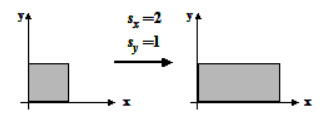
\includegraphics[width=.6\textwidth]{escala}
	\caption{Escalonamento com Sx=2 eS y=1.}
	\fonte{\cite{lapix_escala}}
	\label{fig:escala}
\end{figure}

O escalonamento pode causar distorções na imagens se nao for feita linearmente, e perda de qualidade caso os valores sejam alterados de forma a aumentar a imagem. É muito usado para padronização de tamanhos, e se o escalonamento for feito com a subtração de valores pequenos, a qualidade da imagem pode ser melhorada. Outra vantagem de escalonar a imagem subtraindo valores é o fato de posteriores processamentos performarem mais rapidamente, pois a imagem apresenta-se menor \cite{drmathew_java_programming}. 


\subsubsection{EQUALIZAÇÃO DE HISTOGRAMA}\label{subsubsec:equalizacao}

O histograma de uma imagem digital é definido como "uma função discreta h(rk)=nk onde  rk é o k-ésimo valor de intensidade e nk  é o número de pixels da imagem com intensidade rk e cujos níveis de intensidade desta imagem estejam no intervalo [0, L - 1]." Os Histogramas são a base para várias técnicas de processamento no domínio espacial, onde sua manipulação pode ser utilizada para realce de imagens, além de fornecer dados estatísticos a seu respeito \cite{gonzalez_woods}.

Em outras palavras, esta técnica realça o contraste da imagem com o objetivo de melhorar a qualidade da imagem em um ponto de vista humano. Do ponto de vista computacional, a equalização examina o intervalo de valores em escala de cinza (ou outra disposição de cores, dependendo da imagem) e tonifica mais a parte que existe mudança abrupta do branco pro preto (ou cinza escuro). O resultado ;e uma imagem com maior contraste entre áreas sombreadas e iluminadas, e contornos, tornando a detecção de padrões mais fácil posteriormente \cite{drmathew_java_programming}. A \autoref{fig:histograma} mostra o resultado depois da aplicação deste procedimento.

\begin{figure}[h]
	\centering
	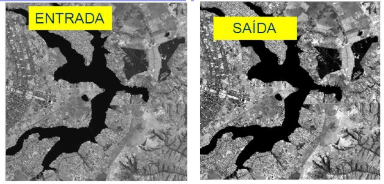
\includegraphics[width=.6\textwidth]{histograma}
	\caption{Exemplo de aplicação de equalização de  histograma.}
%	\fonte{\cite{lapix_escala}}
	\label{fig:histograma}
\end{figure}



\subsubsection{SEGMENTAÇÃO}\label{subsubsec:segmentacao}

Em visão computacional, segmentação se refere ao processo recortar uma imagem digital, ou seja, recolher um conjunto de pixels, para simplificar, mudar a representação de uma imagem ou extrair áreas relevantes para facilitar a sua análise. 

Como resultado, cada um dos pixels em uma mesma região é similar com referência a alguma característica ou propriedade computacional, tais como cor, intensidade, textura ou continuidade. Este processo ~e pr~e requisito para que reconhecimentos de objetos tenham grandes chances de sucesso \cite{gonzalez_woods}.

\subsubsection{CLASSIFICAÇÃO}\label{subsubsec:classificacao}

Segundo \cite{edinburgh_classifier}, classificação de imagem contextual é um tópico de reconhecimento de padrões em  Visão Computacional. Chama-se "contextual" pois significa que esta abordagem é focada na proximidade com os pixels e sua relação com o "classificador", (contemplado na seção \autoref{subsubsec:elem_haar}). É utilizado efetivamente na detecção de objetos e também pode ser aplicado para a detecção de faces em uma imagem.


%============================================================================================================


\section{DETECÇÃO DE FACES COM CARACTERÍSTICAS HAAR}\label{sec:deteccao}

Um classificador HAAR pode ser treinado para detectar vastos tipos de objetos rígidos, definidos, como carros, motos ou partes do corpo humano como olhos ou boca, com altas taxas de sucesso. Não é muito eficiente em reconhecer objetos com ramos tipo arvores, mãos ou objetos camuflados ou contendo pouca textura, contorno e sub-regiões que variam em cor e iluminação \cite{drmathew_java_programming}.

Um classificador bem treinado pode envolver \textit{milhares} de fotos de alta qualidade com imagens positivas. Para a detecção de faces, isto significa imagens de reostos tiradas de perto que devem ter posições similares com muito pouca variação de fundo (\textit{background} \textit{variation}). Olhos bocas e narizes devem estar na mesma posição em todas as fotos, e estas devem ser do mesmo tamanho. Também é necessário treinar o classificador com um número similar de imagens negativas (isto é, sem rostos).

Existem diversas bibliotecas com classificadores pré-treinados para diferentes objetos, incluindo faces.


\subsection{CARACTERÍSTICAS HAAR (\textit{HAAR FEATURES}) }\label{subsubsec:elem_haar}

Os classificadores Haar (ou cacarcterísticas de haar, ou filtro haar) recebem esse nome pela sua similaridade com a \textit{Haar wavelet} (ou ondulação Haar), que consiste em uma sequencia de funções quadradas redimensionadas quem formam uma familia de ondulações das mais simples possíveis.

 \begin{figure}[h]
 	\centering
 	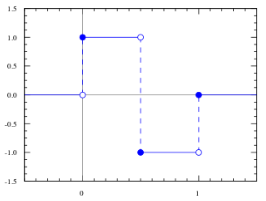
\includegraphics[width=.6\textwidth]{haarwavelet}
 	\caption{Um exemplo de \textit{Haar wavelet}}
 	%	\fonte{\cite{lapix_escala}}
 	\label{fig:haarwavelet}
 \end{figure}

Características Haar são basicamente imagens treinadas e usadas para achar objetos similares em outras imagens. Viole e Jones em seu algorítimo \textit{Haar Cascades}, contemplado na seção seguinte, classificadores retangulares costumam a ser usados. Cada classificador pode indicar a existência ou a ausência de uma característica em outra imagem. A maior motivação para o uso de características de um objeto ao invés do uso de pixel, é que a velocidade da análise de uma imagem baseada no conjunto de sua principais características é muito maior do que a an;alise baseada sobre seus pixels, devido ao fato do numero de características ser substancialmente inferior em relação ao número de pixels \cite{gustavo_cascata}.

A \autoref{fig:haarfeatures} mostra um classificador Haar em ação.

 \begin{figure}[h]
	\centering
	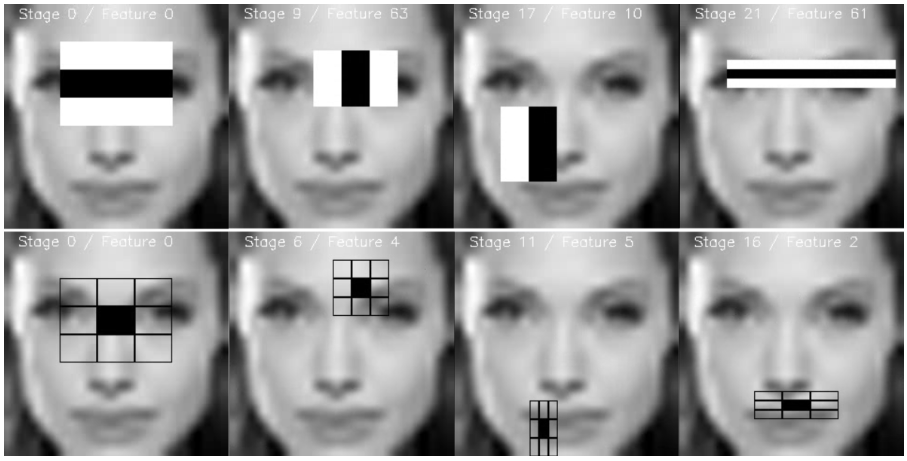
\includegraphics[width=.6\textwidth]{haarfeatures}
	\caption{Classificadores Haar representando características relevantes face}
	\fonte{Biblioteca OpenCV}
	\label{fig:haarfeatures}
\end{figure}

Estes padrões retangulares podem ser escalonados para que caracterísricas de diferentes tamanhos na imagem possam ser detectados usando a mesma abordagem.


\subsection{ALGORÍTIMO VIOLA-JONES (\textit{HAAR CASCADES CLASSIFIER}) }\label{subsubsec:violajones}

O \textit{framework} de detecção de objetos Viola-Jones, apelidado em inglês de \textit{Haar Cascades Classifier}, ou em português Cascata de Classificadores Haar \cite{gustavo_cascata}, foi o primeiro algorítimo de detecção a fornecer detecção de objetos com taxas de sucesso competitivas e em tempo real. Foi proposto em 2001 por Paul Viola e Michael Jones. Apesar de poder detectar uma variedade de classes de objetos, foi desenhada com o objetivo primordial de detectar faces.

Com a utilização das características Haar, o objetivo a ser alcançado é classificar corretamente um dado objeto a partir do conjunto de suas principais características. 

De acordo com \cite{drmathew_java_programming}, o algorítimo funciona com o uso de integrais que é rápida e eficiente, e ainda é possível reduzir drasticamente o numero de atributos que precisam ser testado para decidir se a imagem contem um objeto (por exemplo uma face). O teste de atributos da imagem são organizados em "cascatas" (também pode ser representado por uma árvore binária), representando o use das integrais e  iterativas. O nó raiz da cascata contém o teste que se provou ser o melhor em encontrar um objeto durante o treino. Se uma imagem nao é rejeitada por este teste entao a imagem vai para o nó com o segundo melhor teste, e assim por diante. Apenas se a imagem alcançar o fim de todos os testes (ou o fim da cascata) sem ser rejeitado, a imagem certamente deverá conter o objeto característico .

O grande ponto negativo é que este algorítimo também detecta os objetos que não são realmente os objetos que se tinha a intensão de detectar\cite{drmathew_java_programming}. Por exemplo, o desenho de um rosto certamente vai ser detectado com uma face original, e este desenho não precisa ser muito bem elaborado. As vezes uma disposição de sombras e regiões luminosas aleatórias podem er detectadas como objetos característicos .






%============================================================================================================


\section{RECONHECIMENTO DE FACES COM ANALISE DE COMPONENTE PRINCIPAL (ACP) }\label{sec:recog_faces}


\subsection{ANALISE DE COMPONENTE PRINCIPAL (ACP)}\label{subsec:acp}


\subsection{ACP PARA \textit{EIGENFACES}}\label{subsec:acp-eigen}

\subsection{TREINAMENTO DA FACE}\label{subsec:treiamento}

\subsection{RECONHECIMENTO DA FACE}\label{subsec:reconhecimento}


%============================================================================================================

\section{CONSIDERAÇÕES FINAIS}\label{sec:revbib_consid_finais}






















